\documentclass[tikz,border=2pt]{standalone}
\usepackage{amsmath}
\usepackage{pgfplots}
\pgfplotsset{compat=1.18}
\usetikzlibrary{arrows.meta}
\begin{document}
% Prisoner's dilemma with v(C,C)=(3,3), v(C,D)=(0,5), v(D,C)=(5,0), v(D,D)=(1,1): feasible set
% V = conv of the four payoff vectors; the part of V with v_1 > 1 and v_2 > 1 (vertices (1,1),
% (13/3,1), (3,3), (1,13/3)) is what the folk theorem sustains for delta close to 1.
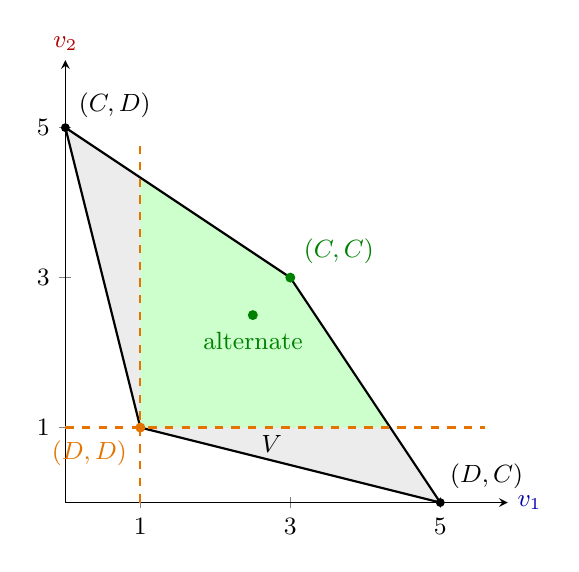
\begin{tikzpicture}[font=\small, >={Latex[length=2mm]}]
  \begin{axis}[
    width=7.2cm, height=7.2cm, axis lines=left,
    xmin=0, xmax=5.9, ymin=0, ymax=5.9,
    xtick={1,3,5}, ytick={1,3,5},
    xlabel={$v_1$}, ylabel={$v_2$},
    xlabel style={blue!70!black, anchor=west, at={(axis description cs:1,0)}},
    ylabel style={red!70!black, rotate=-90, anchor=south, at={(axis description cs:0,1)}},
    clip=false, every tick label/.append style={font=\small}]
    % feasible set V
    \fill[gray!15] (axis cs:1,1) -- (axis cs:5,0) -- (axis cs:3,3) -- (axis cs:0,5) -- cycle;
    % part strictly above the stage Nash payoff (1,1)
    \fill[green!20] (axis cs:1,1) -- (axis cs:13/3,1) -- (axis cs:3,3) -- (axis cs:1,13/3) -- cycle;
    \draw[thick] (axis cs:1,1) -- (axis cs:5,0) -- (axis cs:3,3) -- (axis cs:0,5) -- cycle;
    % thresholds
    \draw[orange!90!black, thick, dashed] (axis cs:1,0) -- (axis cs:1,4.85);
    \draw[orange!90!black, thick, dashed] (axis cs:0,1) -- (axis cs:5.6,1);
    % payoff vectors
    \fill (axis cs:0,5) circle (1.6pt);
    \fill (axis cs:5,0) circle (1.6pt);
    \fill[green!50!black] (axis cs:3,3) circle (1.8pt);
    \fill[green!50!black] (axis cs:2.5,2.5) circle (1.8pt);
    \fill[orange!90!black] (axis cs:1,1) circle (1.8pt);
    \node[anchor=south west] at (axis cs:0.05,5.0) {$(C,D)$};
    \node[anchor=south west] at (axis cs:5.0,0.05) {$(D,C)$};
    \node[green!50!black, anchor=south west] at (axis cs:3.05,3.05) {$(C,C)$};
    \node[green!50!black, anchor=north] at (axis cs:2.5,2.4) {alternate};
    \node[orange!90!black, anchor=north east] at (axis cs:0.95,0.95) {$(D,D)$};
    \node[anchor=center] at (axis cs:2.75,0.78) {$V$};
  \end{axis}
\end{tikzpicture}
\end{document}
